\section{Appendix}

  \subsection{Appendix A}
    \label{sec:AppendixA}
    \begin{figure}[H]
      \centering
      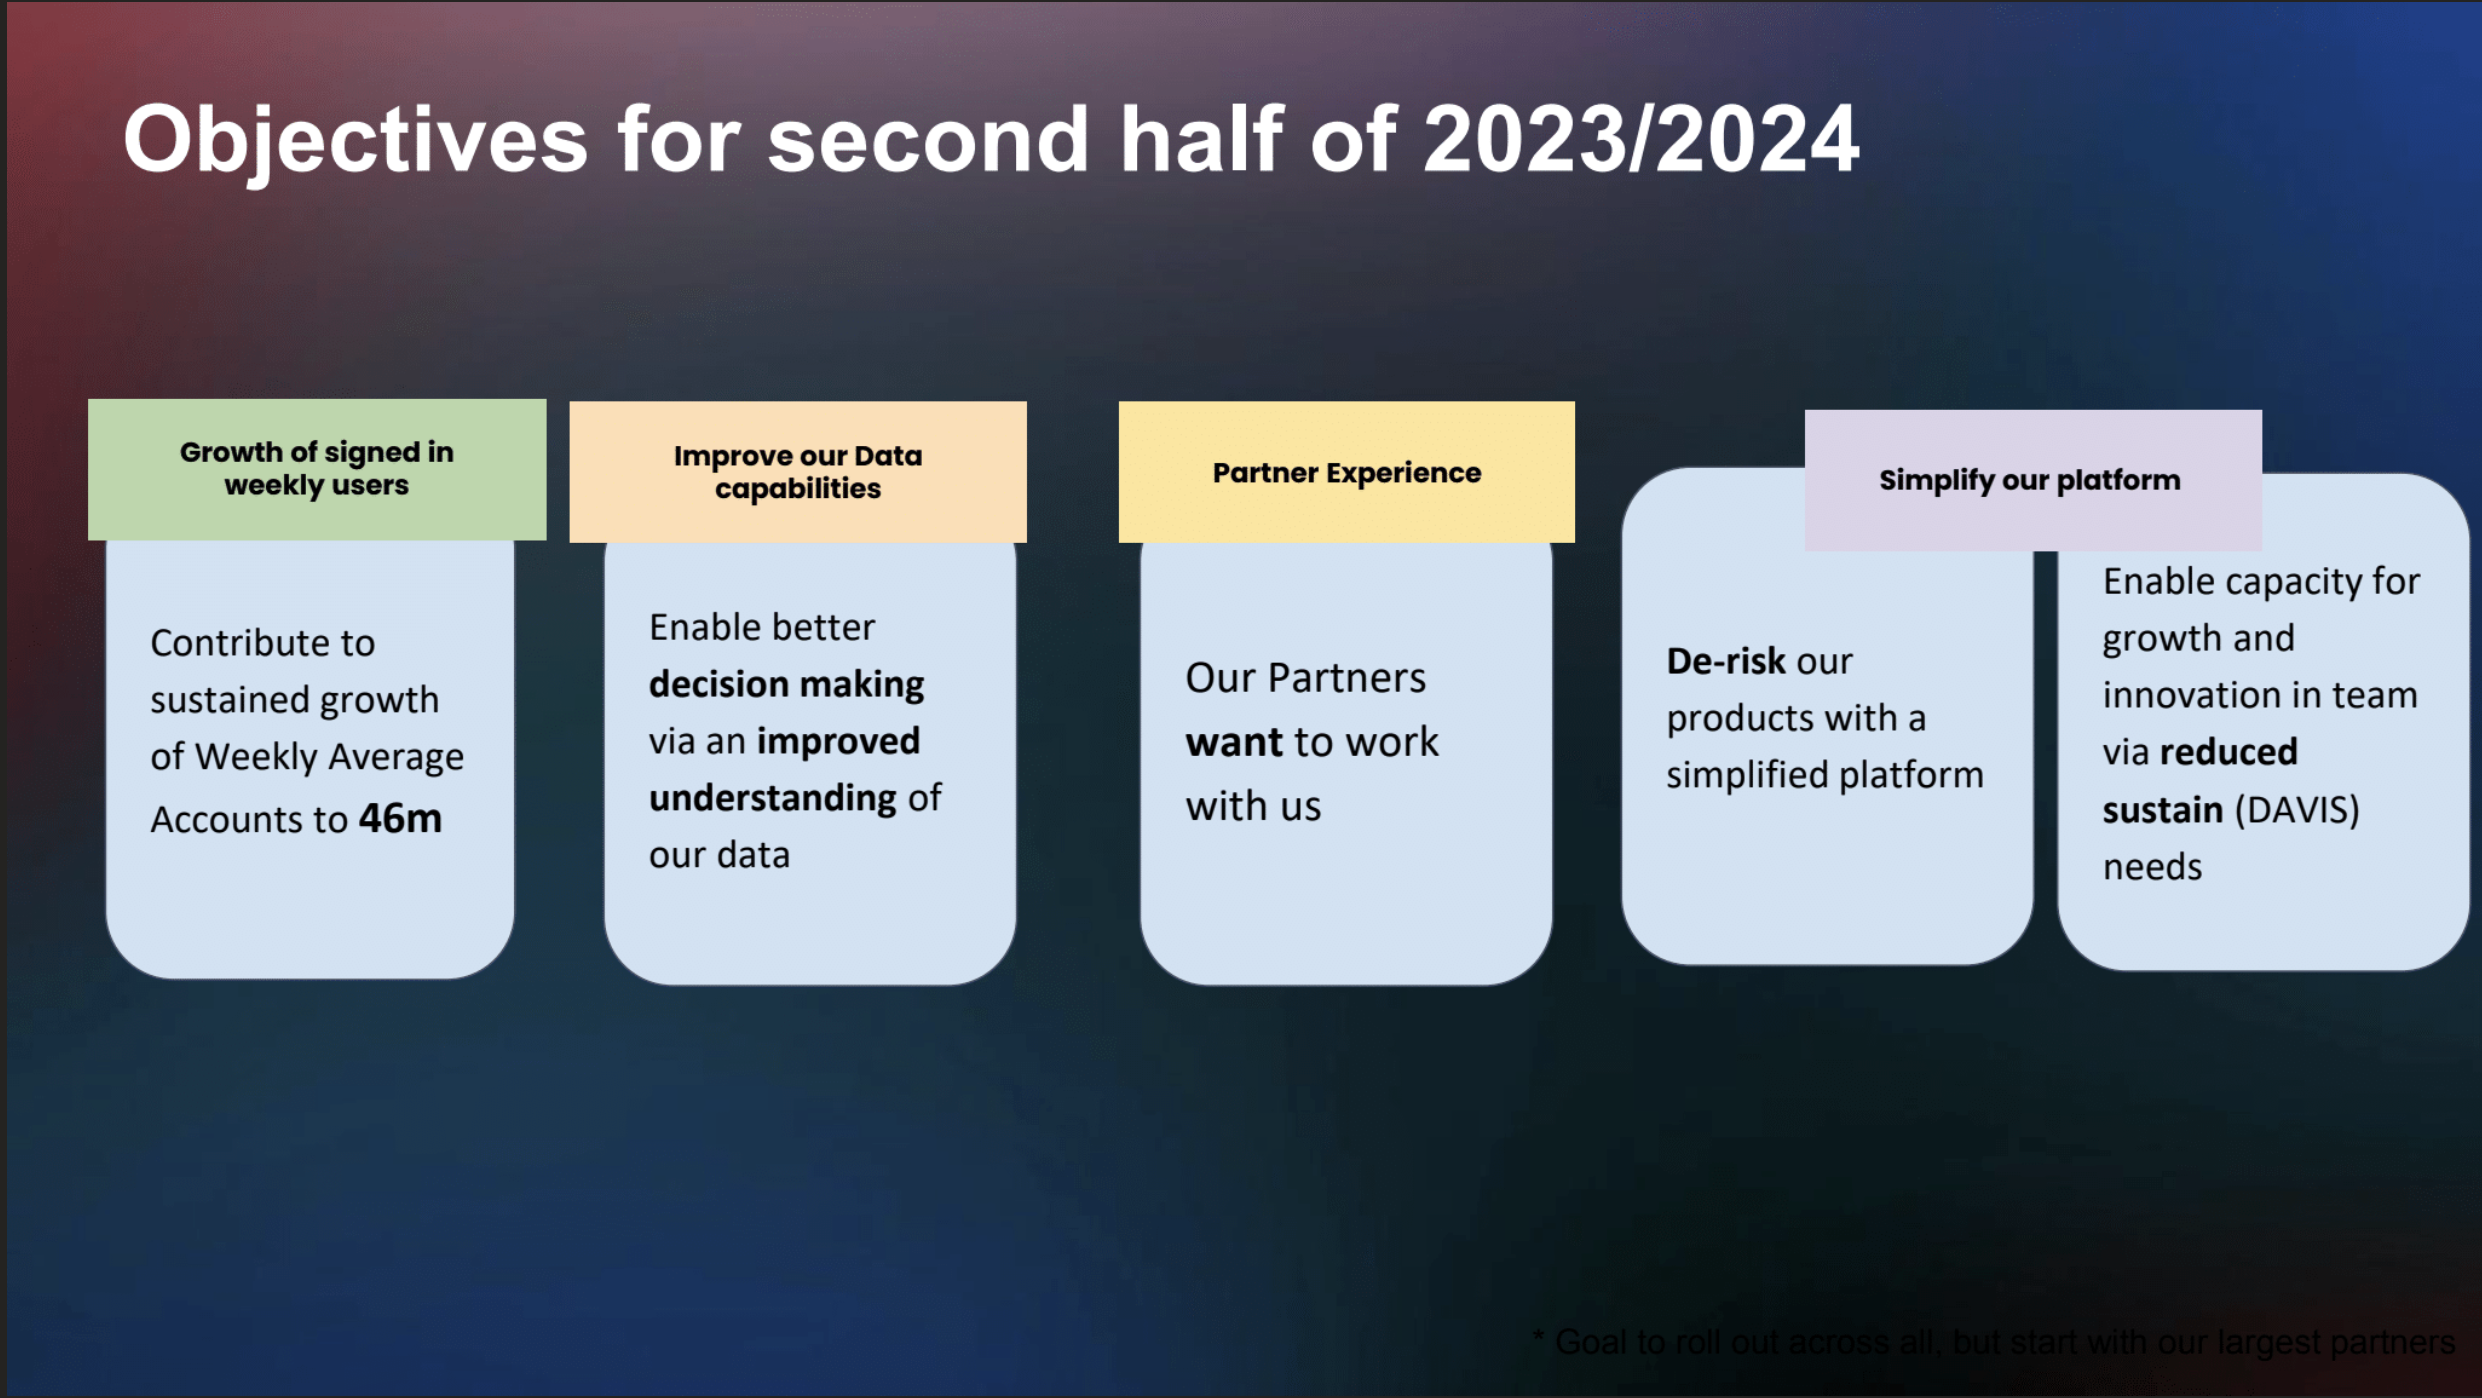
\includegraphics[width=12cm]{assets/appendix/partnershipsObjectives.png}
      \caption{Image taken from a presentation given at a partnerships context setting event (BBC Partnerships, 2023).}
      \label{fig:partnershipsObjectives}
    \end{figure}

  \newpage
  \subsection{Appendix B}
    \label{sec:AppendixB}
    \begin{figure}[H]
      \centering
      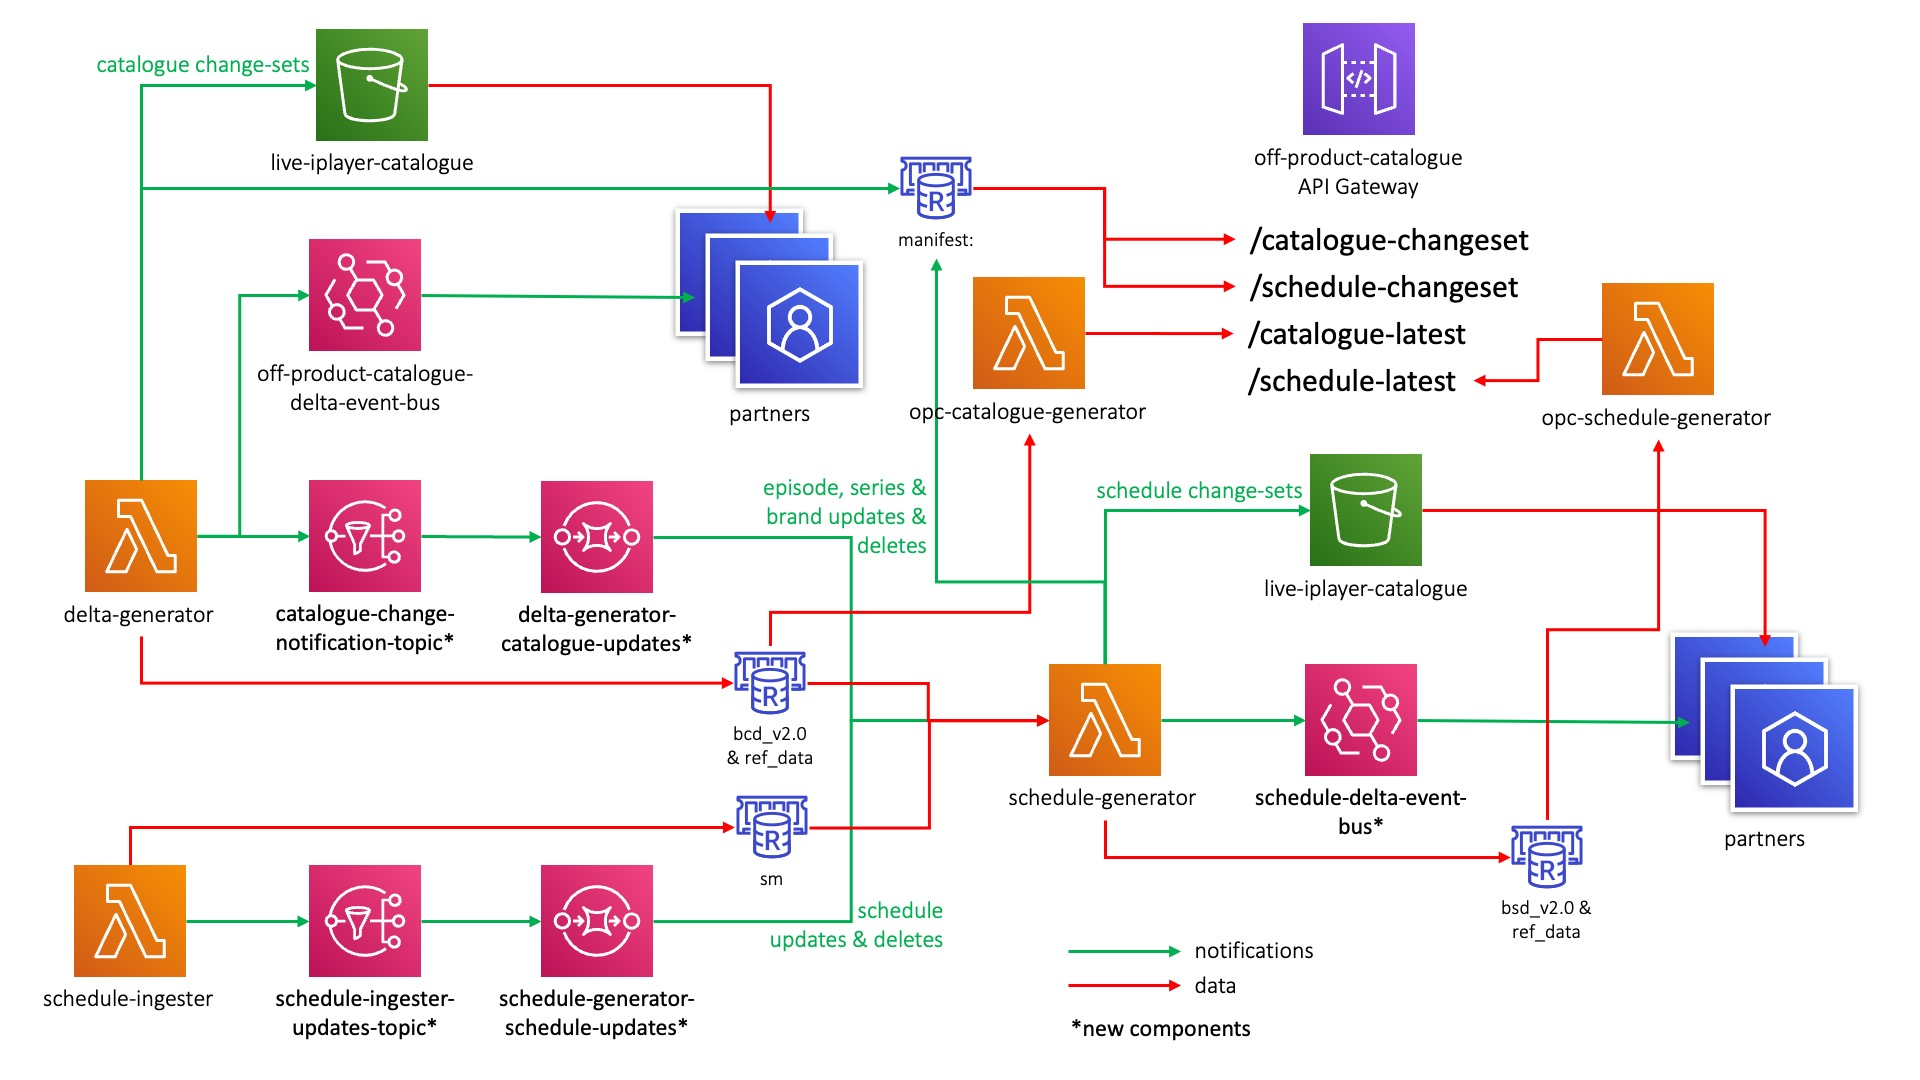
\includegraphics[width=12cm]{assets/appendix/initialDesign.jpg}
      \caption{Full diagram of design for schedules pipeline, including future notifications to partners work (Lloyd, 2023).}
      \label{fig:fullSpikeDesign}
    \end{figure}


  \newpage
  \subsection{Appendix C}
    \label{sec:AppendixC}
    \begin{figure}[H]
      \centering
      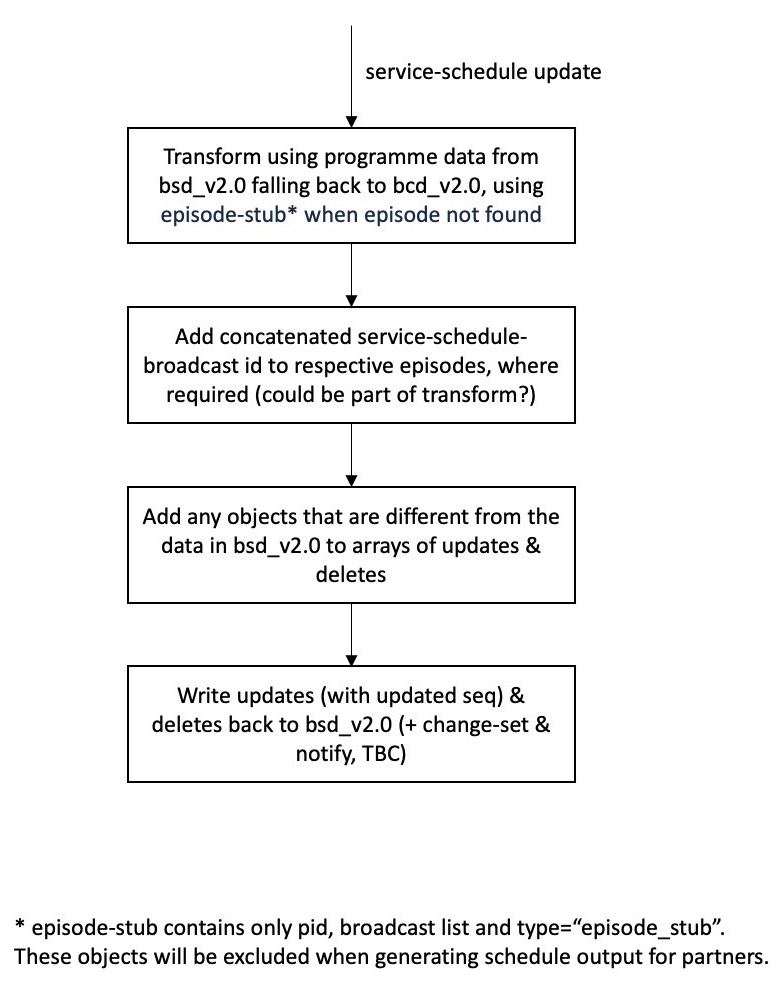
\includegraphics[width=6cm]{assets/initialDesign/scheduleUpdate.jpeg}
      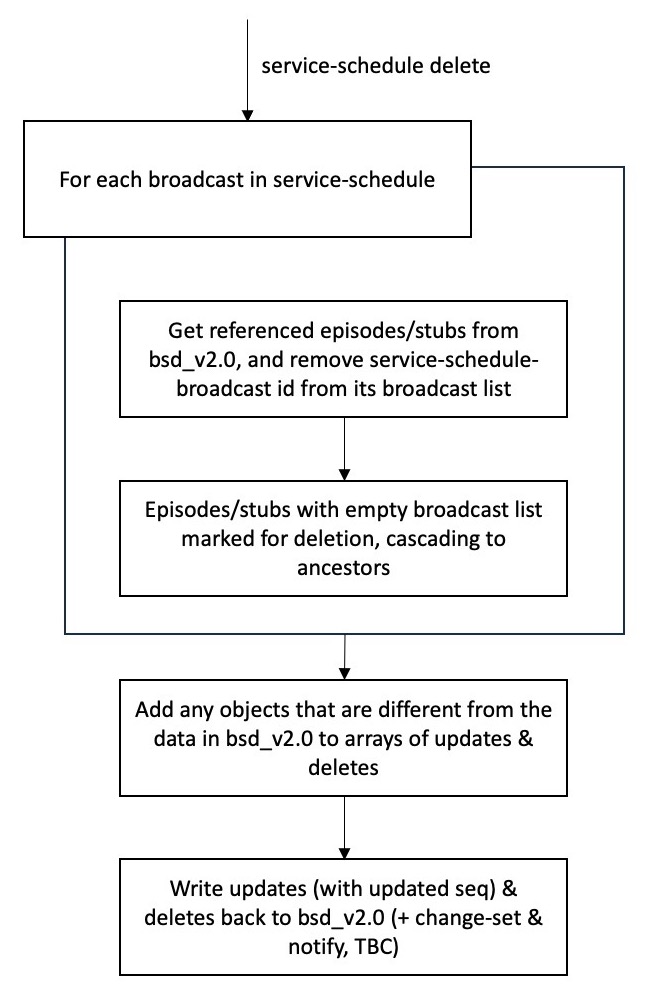
\includegraphics[width=6cm]{assets/initialDesign/scheduleDelete.jpeg}
      \caption{Flow diagrams for schedule events (Lloyd, 2023).}
      \label{fig:initialDesignSchedules}
    \end{figure}


    \begin{figure}[H]
      \centering
      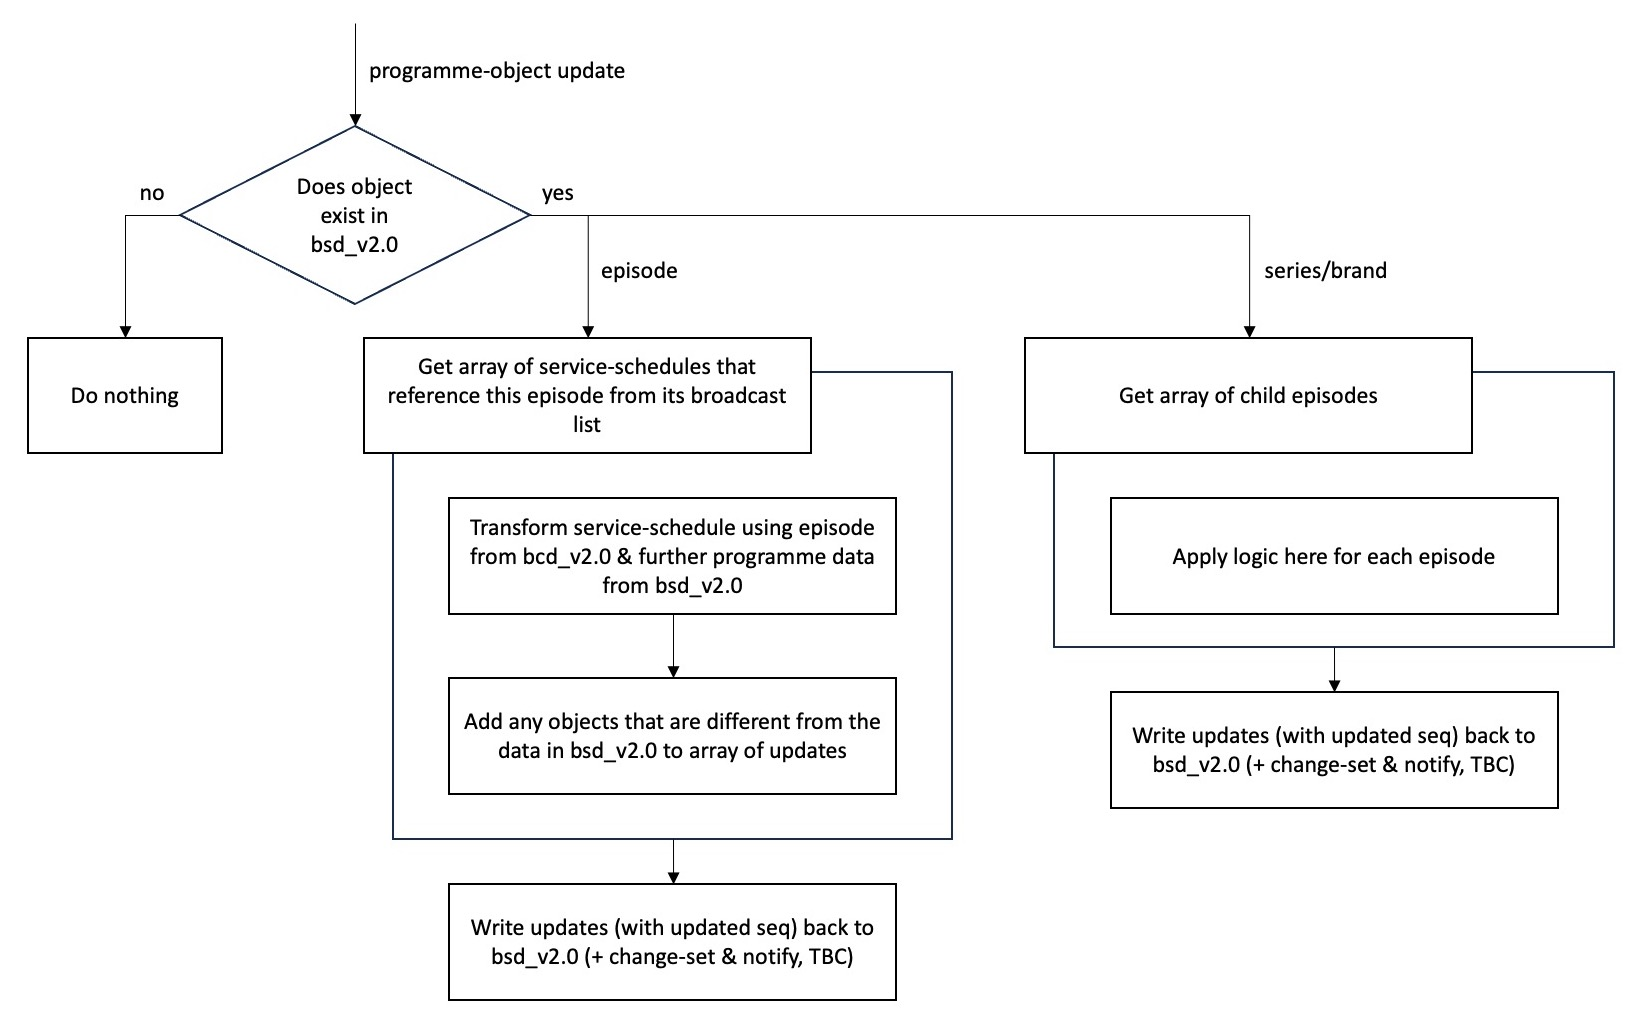
\includegraphics[width=12cm]{assets/initialDesign/programmeUpdate.jpg}
      \caption{Flow diagram for catalogue/programme events (Lloyd, 2023).}
      \label{fig:initialDesignProgrammes}
    \end{figure}

  
  \newpage
  \subsection{Appendix D}
    \label{sec:AppendixD}
    \begin{figure}[H]
      \centering
      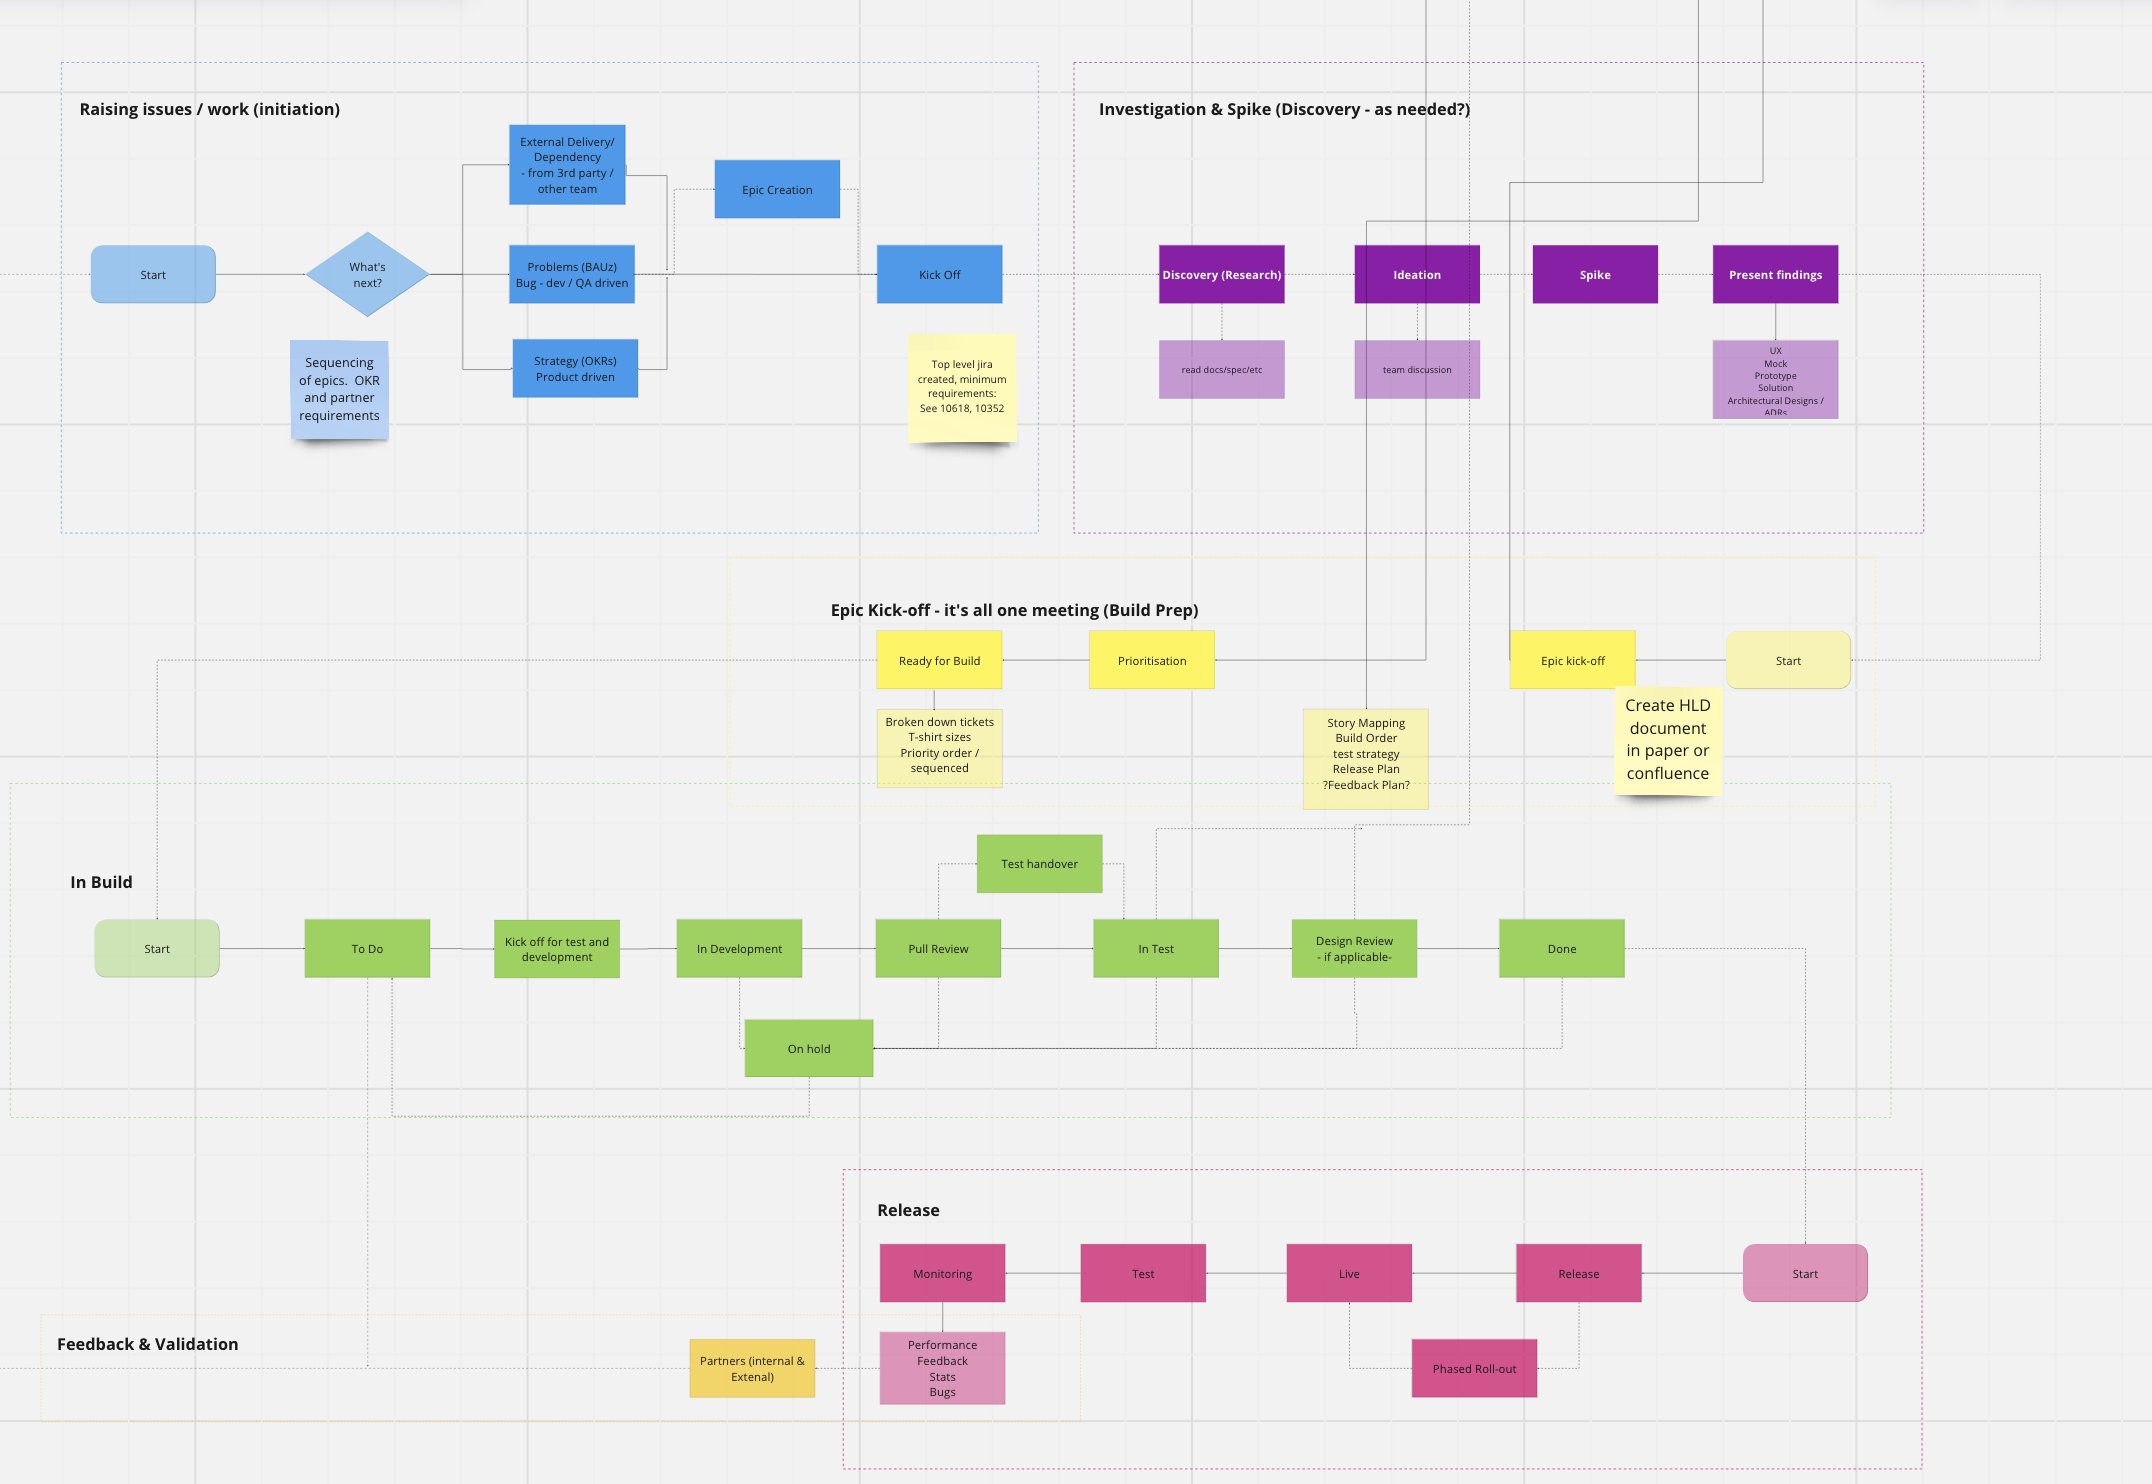
\includegraphics[width=12cm]{assets/workflow/fullWorkflow.png}
      \caption{Full ways of working flow diagram used by SpaceChimp.}
      \label{fig:fullWorkflow}
    \end{figure}
